%!TEX TS-program = xelatex
\documentclass[final]{beamer}

\usepackage[T1]{fontenc}
\usepackage{lmodern}
\usepackage[size=custom,width=120,height=85,scale=1.0]{beamerposter}
\usetheme{gemini}
\usecolortheme{labsix}
\usepackage{graphicx}
\usepackage{booktabs}
\usepackage{tikz}
\usepackage{pgfplots}
\pgfplotsset{compat=1.14}
\usepackage{anyfontsize}
\usepackage{tabularray}
\usepackage{setspace}

\newlength{\sepwidth}
\newlength{\colwidth}
\setlength{\sepwidth}{0.025\paperwidth}
\setlength{\colwidth}{0.3\paperwidth}

\newcommand{\separatorcolumn}{\begin{column}{\sepwidth}\end{column}}
\title{Watts Humphrey}

\author{Yasin Ahmadi}

\institute[shortinst]{KNTU}

\footercontent{
  \href{https://en.kntu.ac.ir}{https://en.kntu.ac.ir}\hfill
  Spring 2024\hfill
  \href{mailto:y.ahmadiahooi@email.kntu.ac.ir}{y.ahmadiahooi@email.kntu.ac.ir}}

\logoleft{
\includegraphics[height=7cm]{images/KNTU.png}}

\begin{document}
\begin{frame}[t]
\begin{columns}[t]
\separatorcolumn
\begin{column}{\colwidth}
  \begin{block}{Biography}
  	\heading{Personal Life \& education}
	Watts Humphrey (1927-2010) was an American software engineer born in Michigan. He suffered from Dyslexia in his childhood.
	\begin{figure}
		\centering
		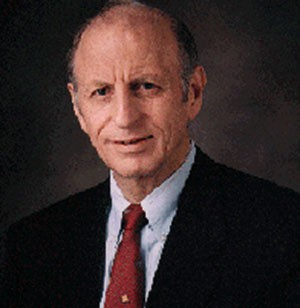
\includegraphics[scale=2.7]{images/WattsHumphrey.png}
		\caption{Watts Humphrey}
	\end{figure}
	He served in the US Navy and received his physics bachelor’s degree from university of Chicago in 1949. He then completed his master’s degree at Illinois Institute of Technology located in Chicago. He also obtained his MBA from university of Chicago.
  	\heading{career}
  	Watts Humphrey made numerous contributions to software engineering field e.g., addressing the problems of software development such as schedule delays, cost overruns, software quality and productivity. In order to honor all his efforts, he was known as the father of software quality. Diagram below shows a summary of his career:
  	\begin{figure}[h]
  		\centering
 		
\includegraphics[scale=0.95]{images/Diag1.png}
  	\end{figure}
  	The SEI had a contract from the Department of Defence (DOD) to provide guidance to the military in the selection of capable software subcontractors. This evolved into the book Managing the Software Process\cite{humphrey1989managing} which describes technical and managerial topics essential for good software engineering.\\
  	Humphrey established the software process program at the SEI, and this led to the development of the software Capability Maturity Model (CMM) and its successors. The CMM is a framework to help an organization to understand its current process maturity and to prioritize improvements. He introduced software process assessment and software capability evaluation methods, and these include CBA/IPI and CBA/SCE. The CMM model and the associated assessment methods were widely adopted by organizations around the world, and their successors are the CMMI Model and SCAMPI appraisal methodology.\\
  	Humphrey focused his later efforts to developing the Personal Software Process (PSP) and the Team Software Process (TSP). These are approaches that teach engineers the skills they need to make and track plans and to produce high-quality software with zero defects. The PSP helps the individual engineer to collect relevant data for statistical process control, whereas the TSP focuses on teams, and the goal is to assist teams to understand and improve their current productivity and quality of their work.
  \end{block}
  \begin{alertblock}{Awards and achievements}
	He has received many awards for his contributions to the computing field.
	\begin{itemize}
	\item He was named the first SEI fellow in 1995 in recognition of his outstanding contribution to the software quality field.
	\item He received the 2003 National Medal in Technology from President George Bush and was named an ACM fellow in 2009 for his outstanding contributions to computing and information technology.
	\item He is the author of 12 books in the software engineering field.
	\end{itemize}
  \end{alertblock}
\end{column}
\separatorcolumn
\begin{column}{\colwidth}

  \begin{block}{Software Process Improvement(SPI)}
	\heading{History}
	Software process improvement focuses on enhancing organizational processes to better achieve business objectives. This could involve enhancing process performance to expedite the development and delivery of high-quality software products. The field traces its roots back to the manufacturing sector, specifically to Walter Shewhart's work on statistical process control in the 1930s.\\
	Deming and Juran refined previous work on quality control, emphasizing that high-quality processes are crucial for producing a high-quality product. They believed that the product's quality is largely determined by the production and support processes. Thus, both the process and the product should be the focus of quality control. Their approach transformed companies with quality issues into ones that could consistently produce high-quality products, leading to cost reductions and increased productivity due to less rework on defective products. Their primary focus was on reducing variability in the manufacturing process.\cite{o2002practical}\\
   \heading{Humphrey's impact}
  	This work was later applied to the software quality field by Watts Humphrey and others at the SEI, leading to the birth of the software process improvement field.
  	\ Software process improvement initiatives aim to enhance an organization’s ability to deliver software quickly, improve quality, and reduce waste. These initiatives, which provide a tangible return on investment, involve changes to work methods and require top management support. The involvement of software engineering staff is crucial, and changes are made based on the strengths and weaknesses of the process. Continuous improvement is sought in every task and activity. Training reinforces the processes, and audits ensure process fidelity. Ultimately, improving software processes enhances software quality.\\
  	The Software Engineering Institute (SEI) developed the Capability Maturity Model (CMM) in the early 1990s as a framework to help software organizations to improve their software process maturity and to implement best practice in software and systems engineering. The SEI believes that there is a close relationship between the maturity of software processes and the quality of the delivered software product. The first version of the CMM was released in 1991, and its successor is the Capability Maturity Model Integration (CMMI®)\cite{chrissis_2011}.\\
  	The SEI maintains data on the benefits that organizations have achieved from using the CMM and CMMI. It has measured the improvements in several categories such as cost, schedule, productivity, quality, customer satisfaction and a return on investment.
  	\begin{block}{Capability Maturity Model Integrated (CMMI)}
  		The Capability Maturity Model Integration (CMMI), developed by the Software Engineering Institute (SEI), is a framework for enhancing software process maturity. It succeeded the earlier Capability Maturity Model (CMM). Both models aim to implement best practices in software and systems engineering. Quality experts recognize a strong link between process maturity and software product quality. To create high-quality software, companies must establish robust software processes. The CMMI assists organizations worldwide in implementing these best practices. It enables management to identify and enhance key processes, which serve as the glue connecting people, procedures, and tools. Process improvement aligns with business goals, ensuring more effective outcomes .\\
  		The CMMI consists of five maturity levels with each maturity level (except level one) consisting of several process areas. Each process area consists of a set of goals, which must be implemented for the process area to be satisfied. The goals are implemented by practices related to that process area, and processes need to be defined and documented. The users of the process need to receive appropriate training to enable them to carry out the process, and processes need to be enforced by independent audits.
  		{\setstretch{2.5}\begin{figure}
  				\begin{tikzpicture}
  					\draw (0,0) -- (12,0) -- (6,5) -- cycle;
  					\node at (.8,3) {\normalsize people};
  					\node[align=left] at (13,3) {\normalsize Procedures\\\normalsize and\\\normalsize Methods};
  					\node at (6,-1.5) {\normalsize Tools and Equipment};
  					\node at (6,2) {\normalsize Process};
  				\end{tikzpicture}
  				\caption{Process as glue for people, procedure and tools}
  				\label{process}
  		\end{figure}}
  	\end{block}
  \end{block}
\end{column}
\separatorcolumn
\begin{column}{\colwidth}
	\begin{block}{Capability Maturity Model Integrated (CMMI)}
	The emphasis on level two of the CMMI is on maturing management practices such as project management, requirements management and configuration management The emphasis on level three of the CMMI is to mature engineering and organization practices. This maturity level includes peer reviews and testing, requirements development and software design. Level four is concerned with ensuring that key processes are performing within strict quantitative limits and adjusting processes, where necessary, to ensure that performance is within these limits. Level five is concerned with continuous process improvement that is quantitatively verified.\\
	Maturity levels may not be skipped in the staged implementation of the CMMI. There is also a continuous representation of the CMMI that allows the organization to focus on improvements to key selected processes. However, in practice, it is often necessary to implement several of the level two process areas before serious work can be done on implementing a process at a higher maturity level. The use of metrics \cite{FE95,gilb_77} becomes more important as an organization matures, as metrics allow the performance of an organization to be objectively judged.
\end{block}
\begin{exampleblock}{PSP and TSP}
	\heading{PSP}
	The Personal Software Process (PSP) is a structured, data-driven approach to software development that aims to enhance the performance of individual engineers. Developed by Watts Humphrey at the SEI, PSP equips engineers with methods and tools to improve their estimation, planning skills, and defect reduction, thereby enabling them to deliver quality projects on time and within budget. The process is divided into three levels: PSP level 1 focuses on estimation and planning, PSP level 2 on design, code reviews, and quality management, and PSP level 3 on larger projects. Overall, PSP helps engineers manage their work effectively and maintain quality control.
	\heading{TSP}
	The Team Software Process (TSP) is a structured approach developed by Watts Humphrey at the Software Engineering Institute (SEI). It aims to enhance the quality and productivity of software teams.Note that Team members must already be familiar with the Personal Software Process (PSP).
	\begin{figure}
		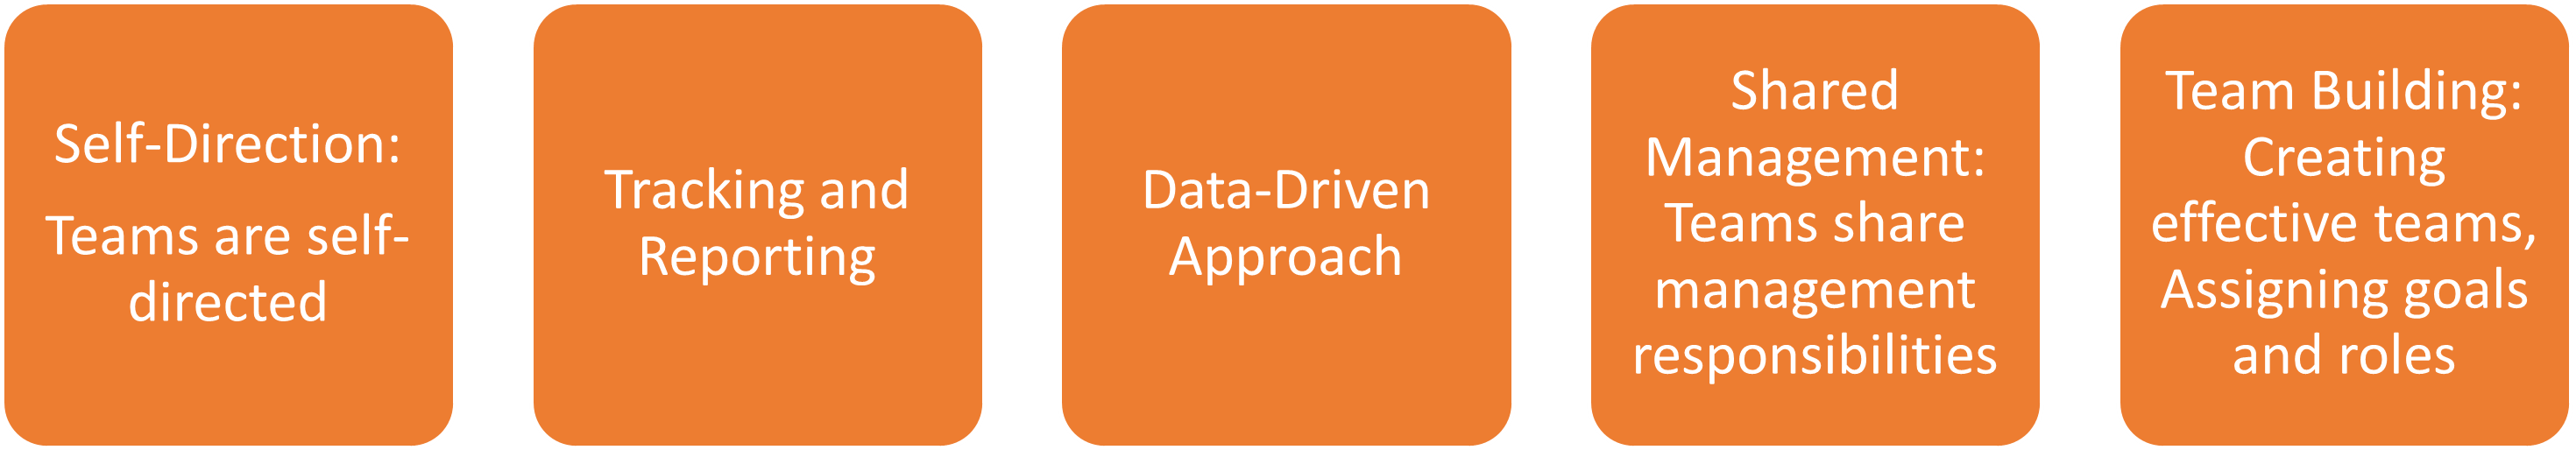
\includegraphics{images/Diag2.png}
		\caption{Key features of TSP}
	\end{figure}
\end{exampleblock}
  \begin{block}{References}
    \nocite{*}
    \footnotesize{\bibliographystyle{plain}\bibliography{all.bib}}
  \end{block}

\end{column}

\separatorcolumn
\end{columns}
\end{frame}

\end{document}
